\section{レポート課題 3rd}
\subsection{課題1}
\subsubsection{問題}
$a = 1.4, b = 0.3$ として、Henon写像のアトラクタを描け。アトラクタへ至るまでの過渡状態は書かなくてよい。
\subsubsection{画像}
\begin{figure}[htbp]
  \centering
  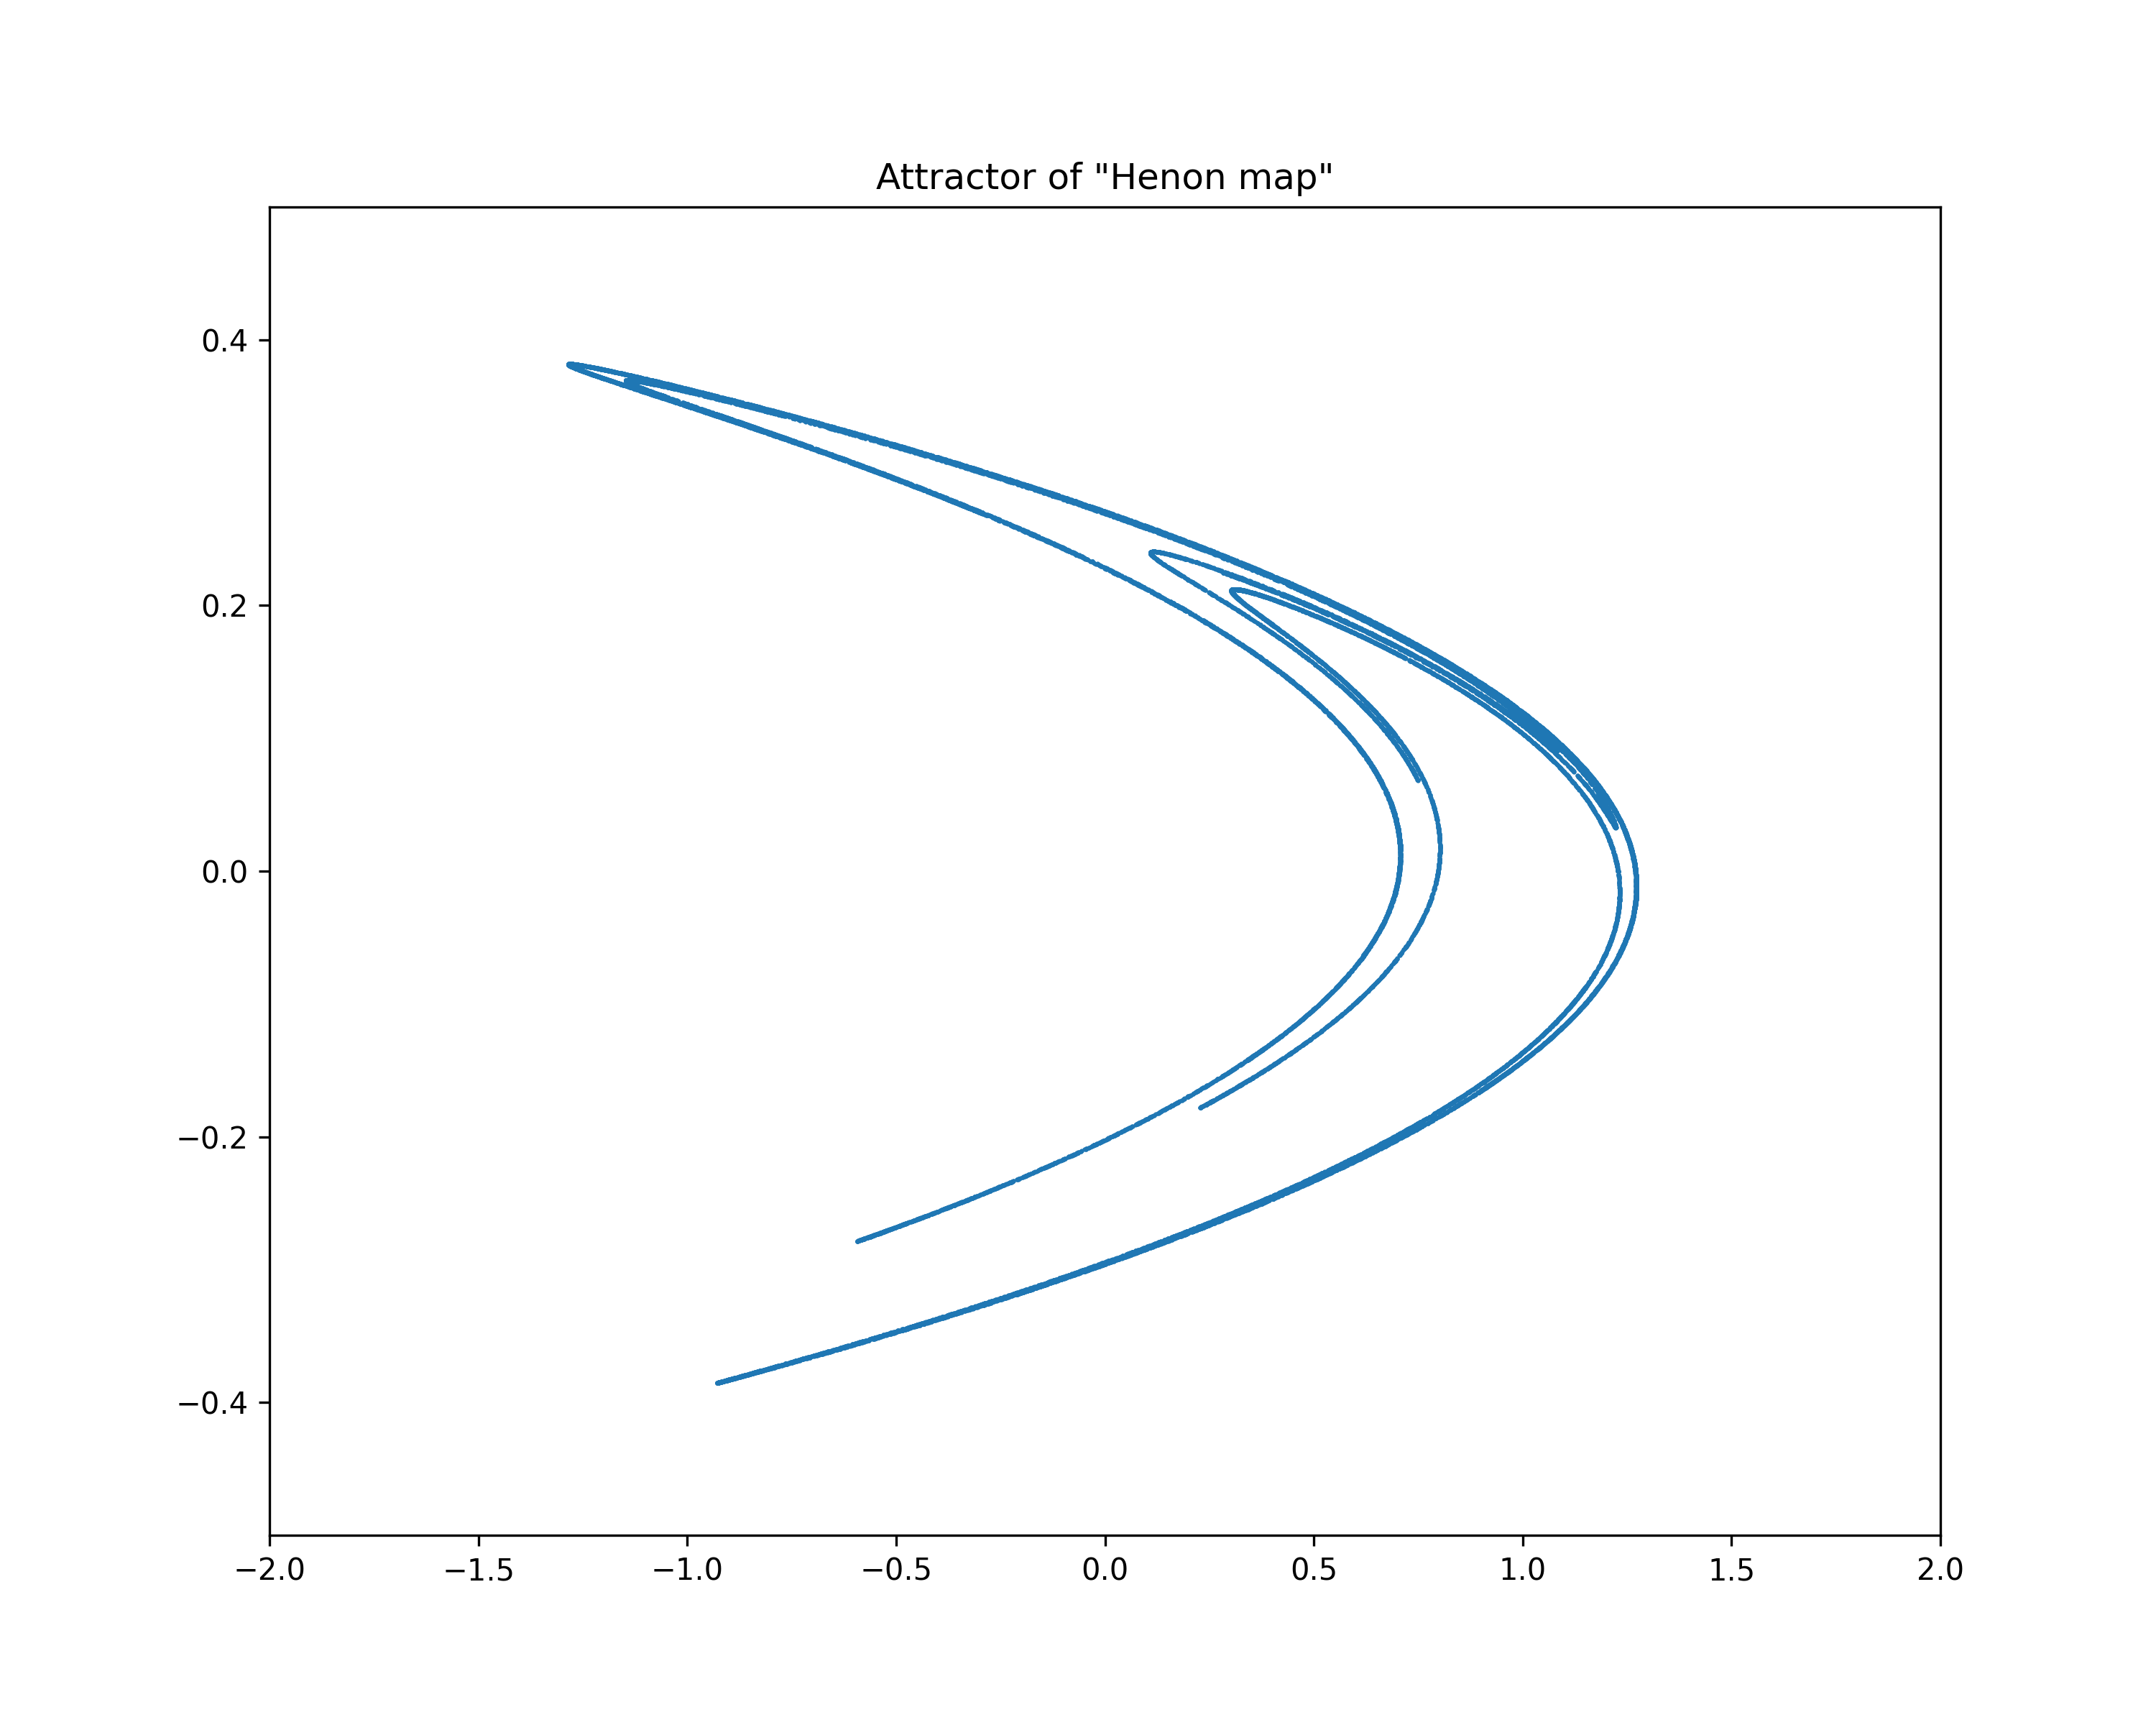
\includegraphics[keepaspectratio, scale=0.5]{images/Problem8/task8_1.png}
\end{figure}
\subsubsection{考察}
漸化式を代入しPythonで実行させた結果、画像のような結果になった。この画像を拡大していくと同様の解軌道を描いていくことが発見できた。そのため、エノン写像にはフラクタル構造があるのではないかと考察した。
\subsubsection{ソースコード}
\begin{lstlisting}[caption=task8-1.py]
  from matplotlib import pyplot as plt
  from random import uniform


  def henon(x: float, y: float):
      return y + 1 - a * x ** 2, b * x


  x = uniform(-1, 1)
  y = uniform(-1, 1)
  a = 1.4
  b = 0.3
  cnt = 30000
  x_array = []
  y_array = []
  for i in range(cnt):
      x, y = henon(x, y)
      if i < 249:
          continue
      x_array.append(x)
      y_array.append(y)
  plt.figure(figsize=(10, 8))
  plt.plot(x_array, y_array, linestyle='None', marker='.', markersize=1)
  plt.title('Attractor of "Henon map"')
  plt.xlim(-2, 2)
  plt.ylim(-0.5, 0.5)
  # plt.show()
  plt.savefig('複雑系科学演習/Week8/images/task8_1', dpi=300)
\end{lstlisting}

\newpage
\subsection{課題2}
\subsubsection{問題}
$b = 0.3$ に固定して、横軸 $a$ 縦軸 $x_n$ の分岐図を描け。$a \in [0, 1.5]$ を $0.01$ 刻みで変化させたときの、$x_n(n = 250から500)$ の点を打つこと。時間とファイルサイズが許すなら、より刻み幅を小さくしてもよい。
\subsubsection{画像}
\begin{figure}[htbp]
  \centering
  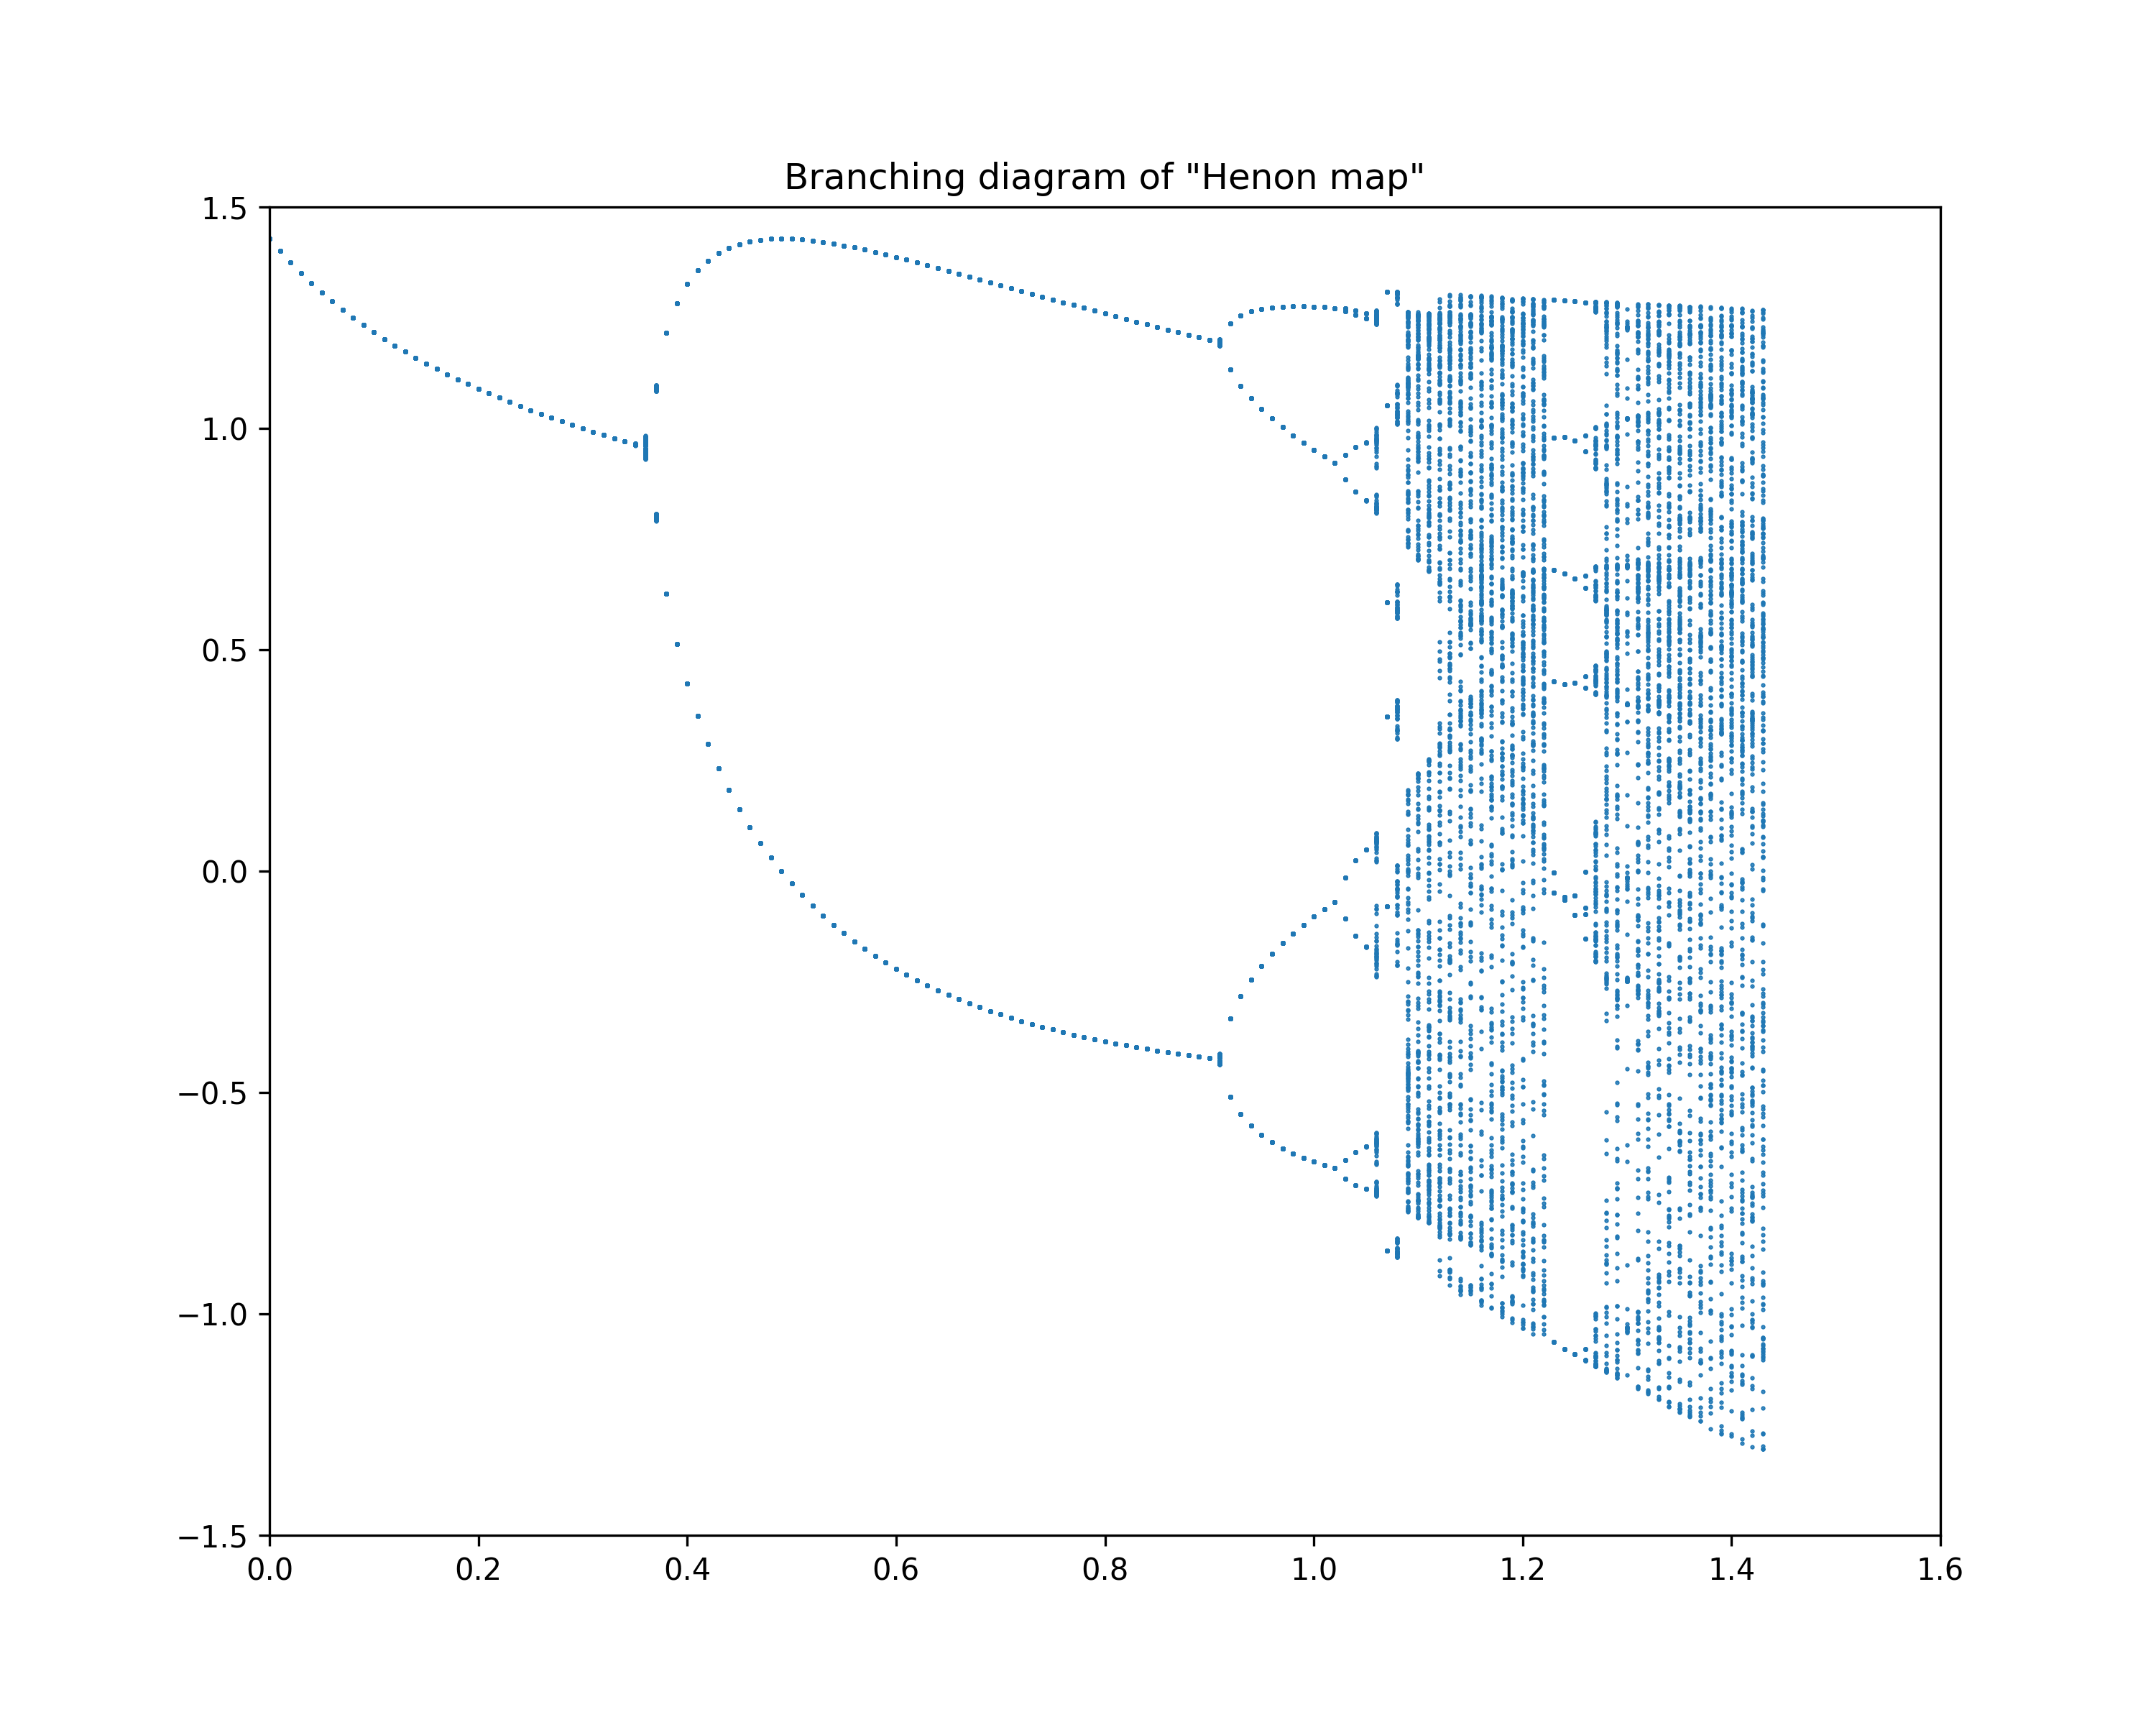
\includegraphics[keepaspectratio, scale=0.5]{images/Problem8/task8_2.png}
\end{figure}
\subsubsection{考察}
考察については次の課題3に記述している。

\subsubsection{ソースコード}
\begin{lstlisting}[caption=task8-2.py]
  from matplotlib import pyplot as plt
  import numpy as np
  from random import uniform


  def henon(a: float, x: float, y: float):
      """エノン写像の(x, y)座標を返す関数"""
      return y + 1 - a * x ** 2, b * x


  a = np.arange(0, 1.5, 0.01, dtype=object)   # 課題2の a の範囲
  b = 0.3                                     # b = 0.3 に固定
  x0 = uniform(-1, 1)                         # ランダムの初期値x0([-1, 1]の範囲)
  y0 = uniform(-1, 1)                         # ランダムの初期値y0([-1, 1]の範囲)
  x_array = []                                # x の値を保存するための配列
  a_array = []                                # a の値を保存するための配列

  for i in a:                                 # 各 a のときの振る舞いを計算する
      x = x0
      y = y0
      for j in range(500):
          x, y = henon(i, x, y)
          if x < -1.5 or 1.5 < x:             # プロットの範囲外なら終了(オーバーフローを避けるため)
              break
          if j < 249:                         # 250 < xn < 500 の範囲外なら配列に入れない
              continue
          x_array.append(x)
          a_array.append(i)

  plt.figure(figsize=(10, 8))
  plt.plot(a_array, x_array, linestyle='None', marker='.', markersize=1)
  plt.title('Branching diagram of "Henon map"')
  plt.xlim(0, 1.6)
  plt.ylim(-1.5, 1.5)
  # plt.show()
  plt.savefig('複雑系科学演習/Week8/images/task8_2', dpi=300)
\end{lstlisting}

\subsection{課題3}
\subsubsection{問題}
問2の分岐図よりわかることは何か?(例えば分岐の種類など)
\subsubsection{考察}
$r = 0.4$ 付近を境に周期倍分岐を起こしていることが読み取れた。